We collect 2050 human-human navigation dialogs, comprising over 7k navigation trajectories punctuated by question-answer exchanges, across 83 MatterPort~\cite{chang:3dv17} houses.\footnote{A demonstration video of the data collection interface: \url{https://youtu.be/BonlITv_PKw}.}
We prompt with initial instructions that are both \textit{ambiguous} and \textit{underspecified}.
An \textit{ambiguous} navigation instruction is one that requires clarification because it can refer to more than one possible goal location.
An \textit{underspecified} navigation instruction is one that does not describe the route to the goal.

\begin{figure}[ht]
\begin{tabular}{ccc}
    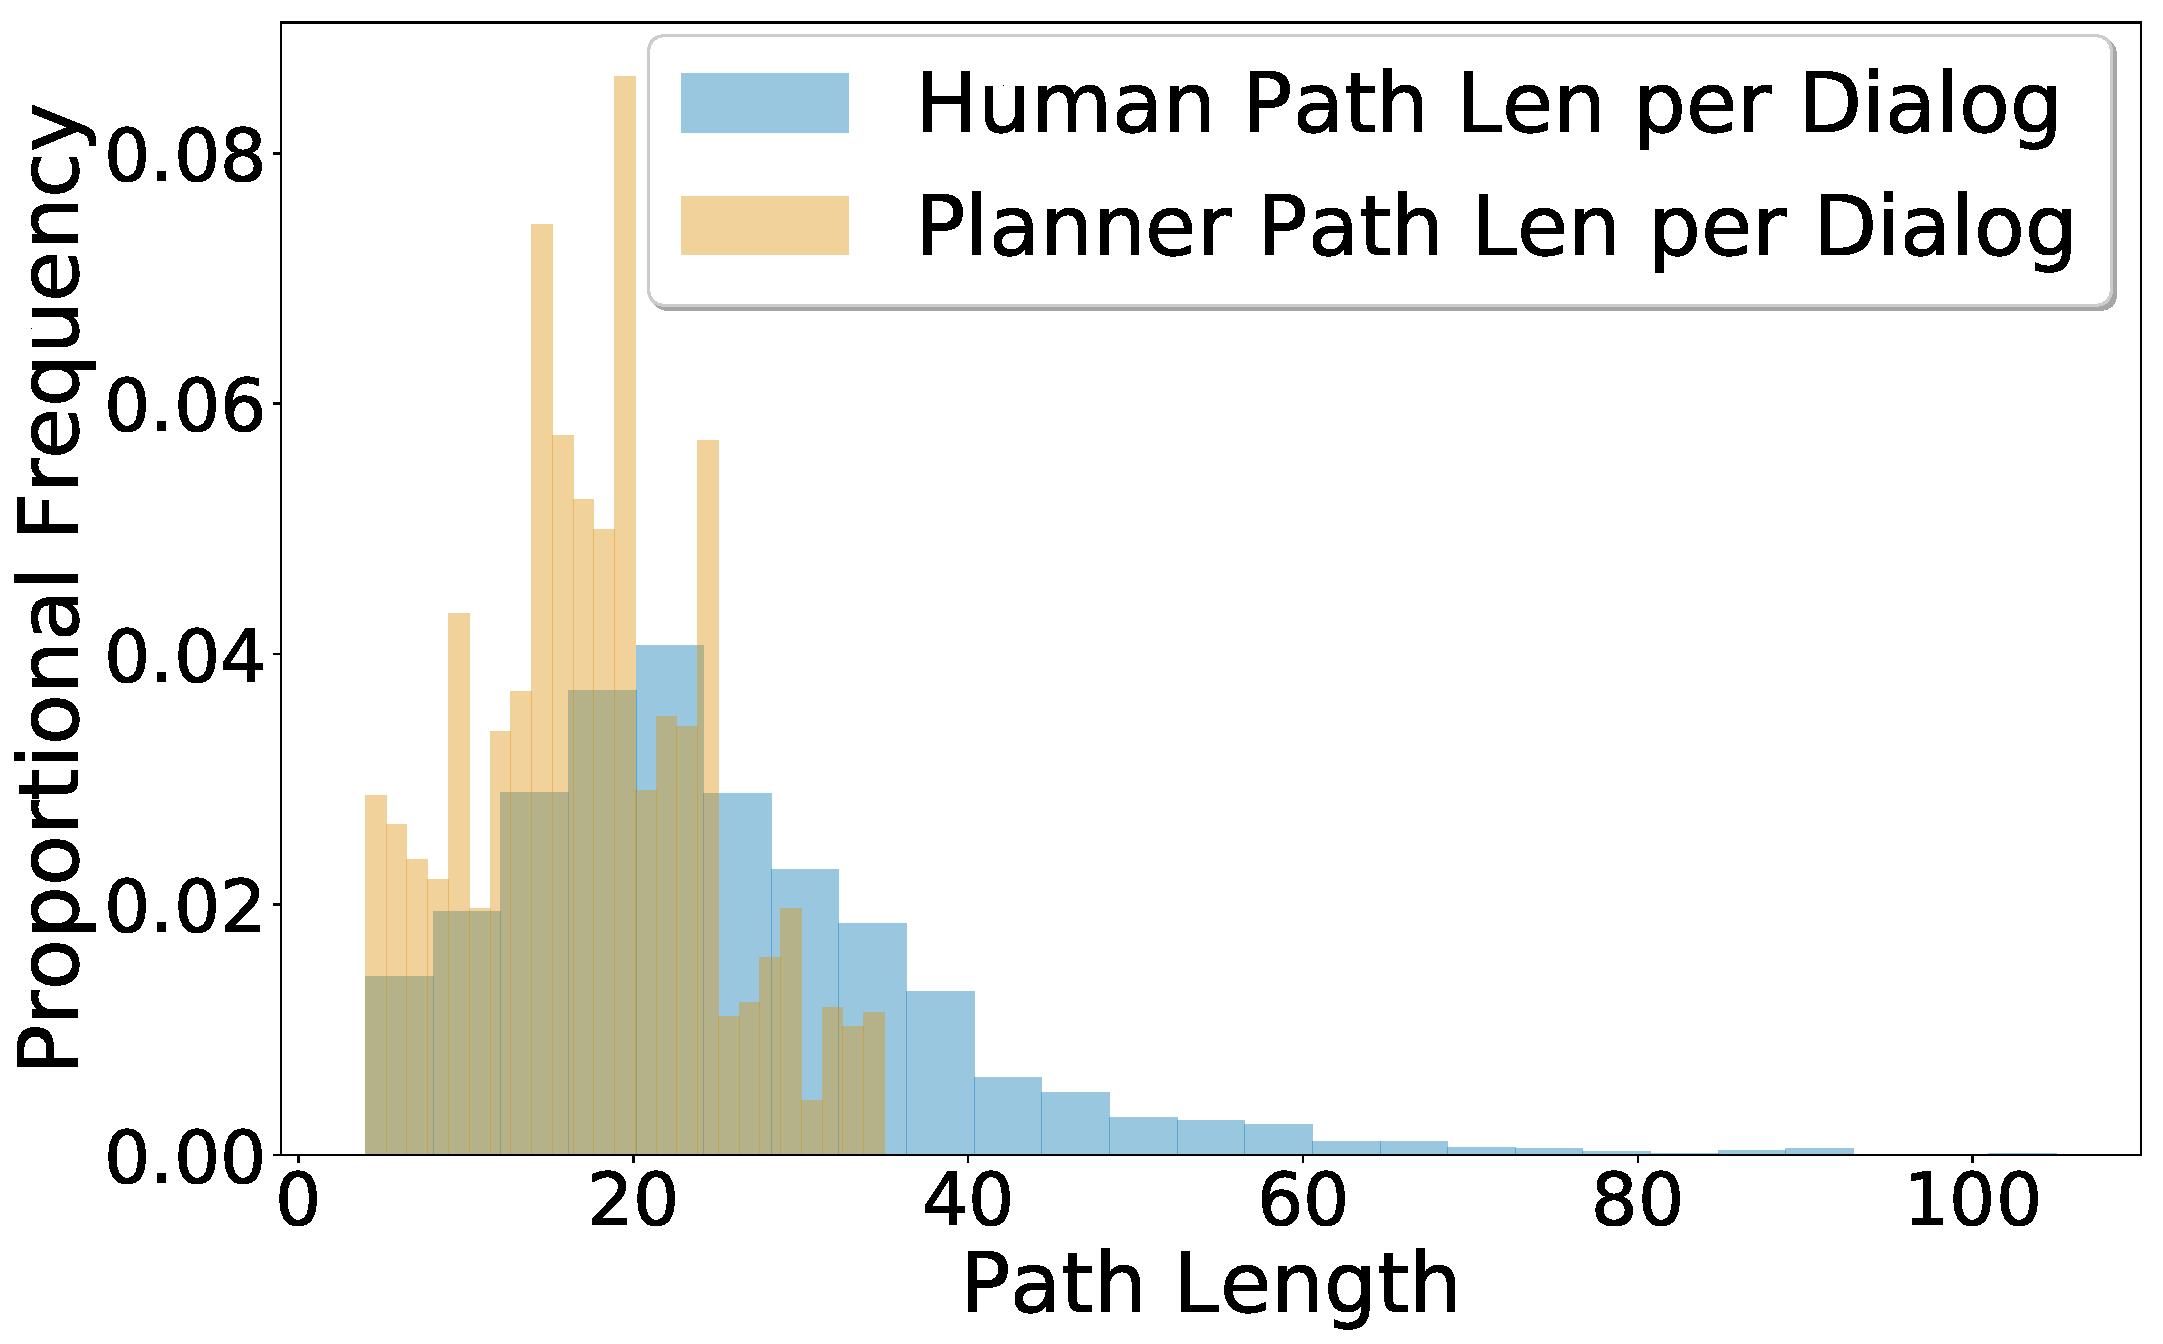
\includegraphics[width=0.3\columnwidth]{figures/player_planner_steps_per_dialog.pdf} &
    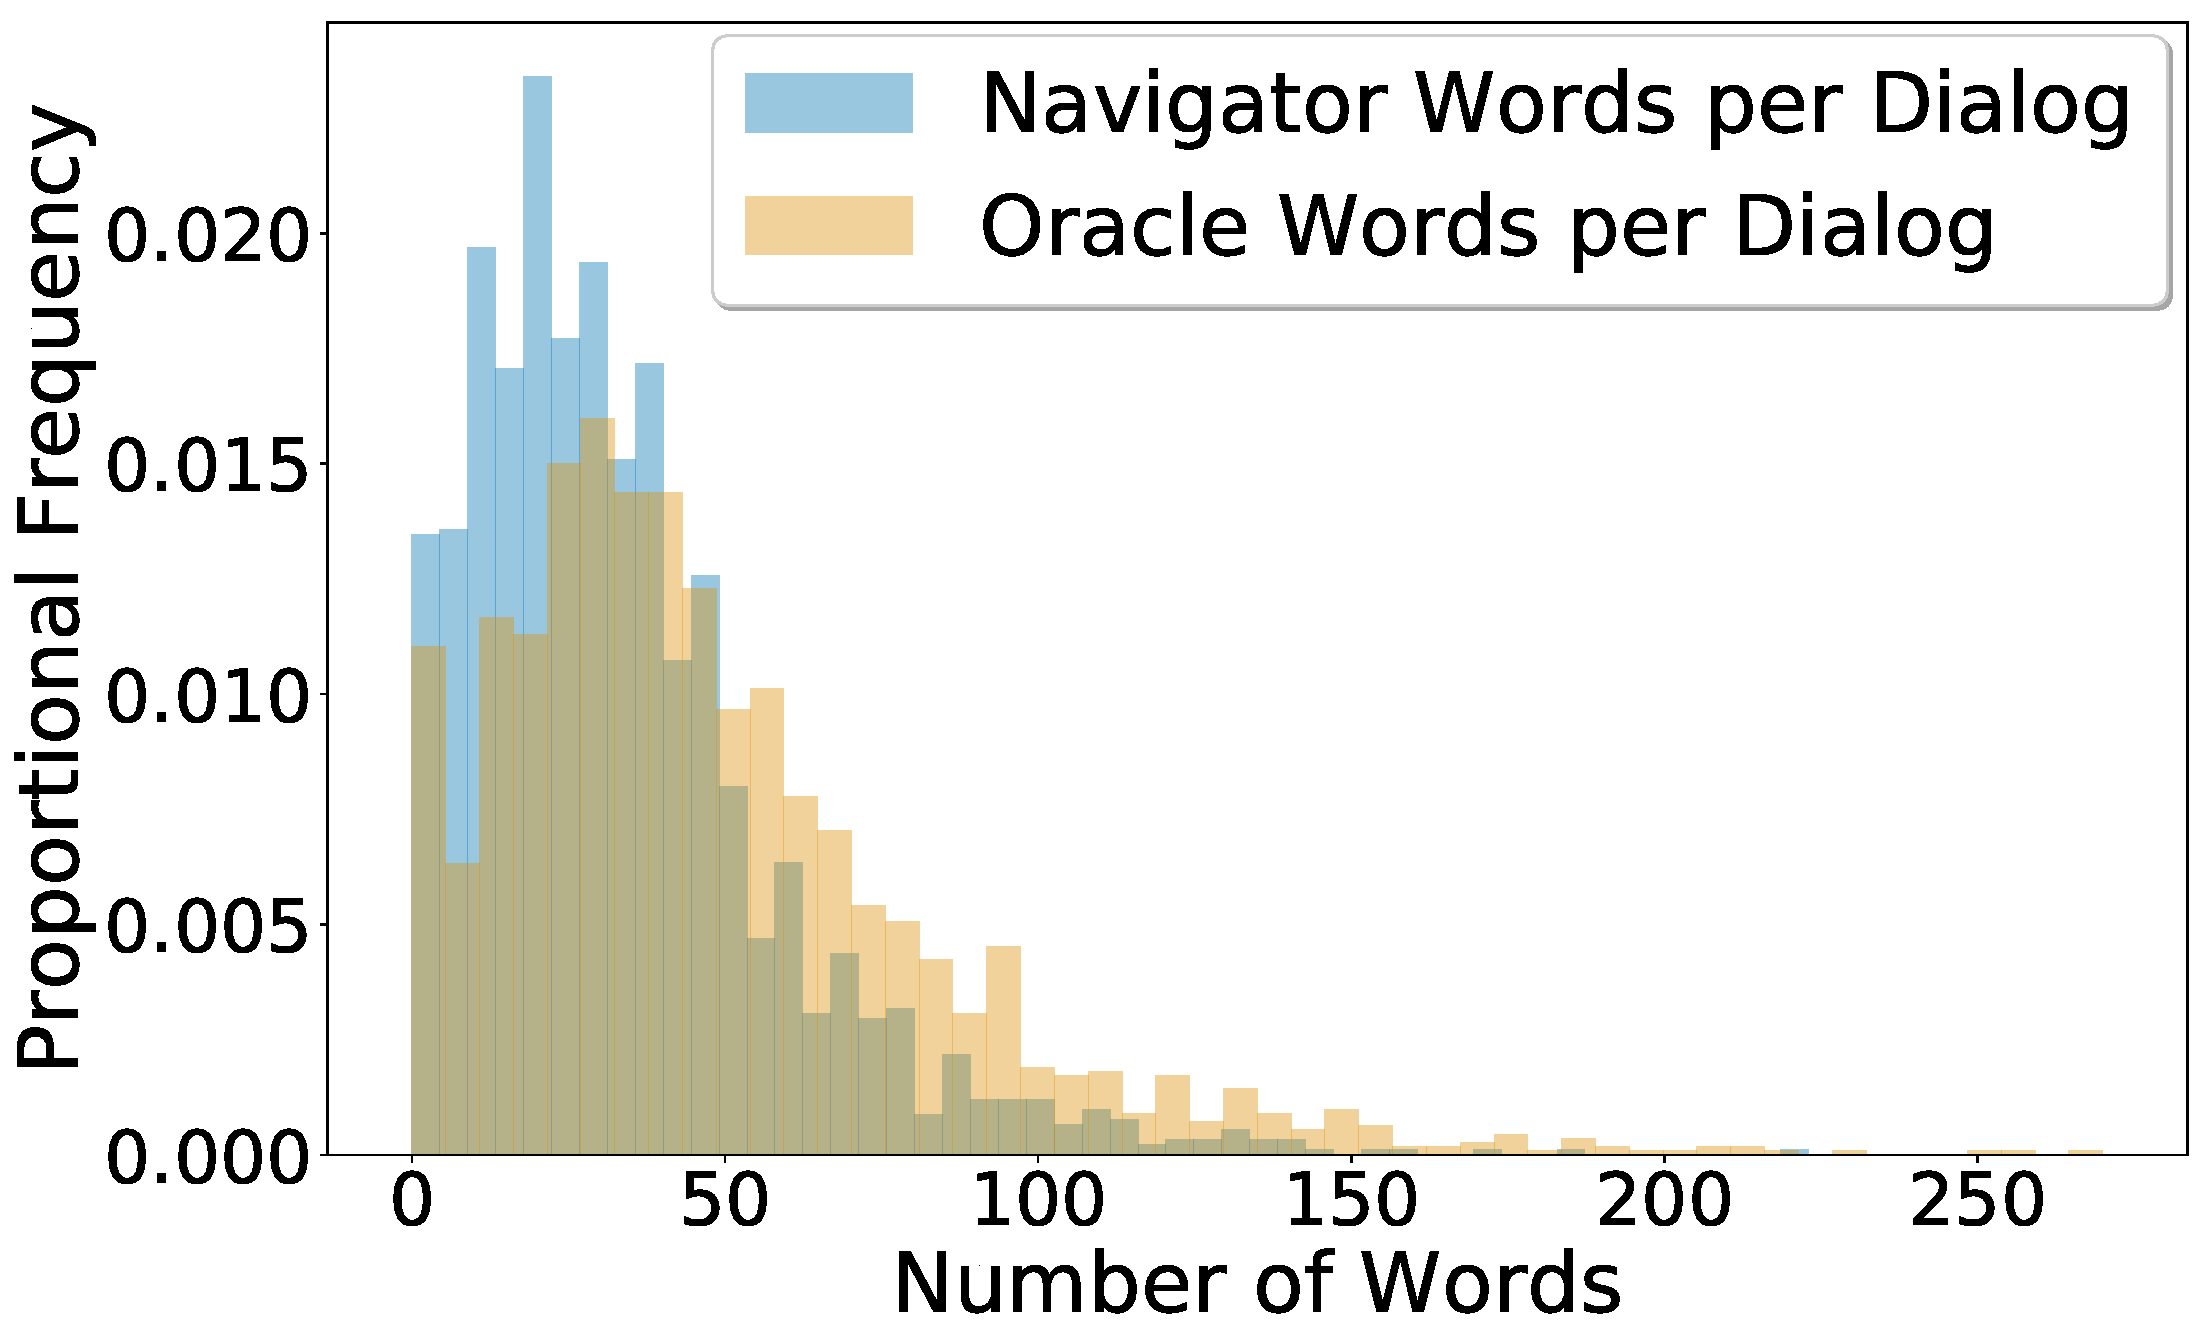
\includegraphics[width=0.3\columnwidth]{figures/nav_ora_words_per_dialog.pdf} &
    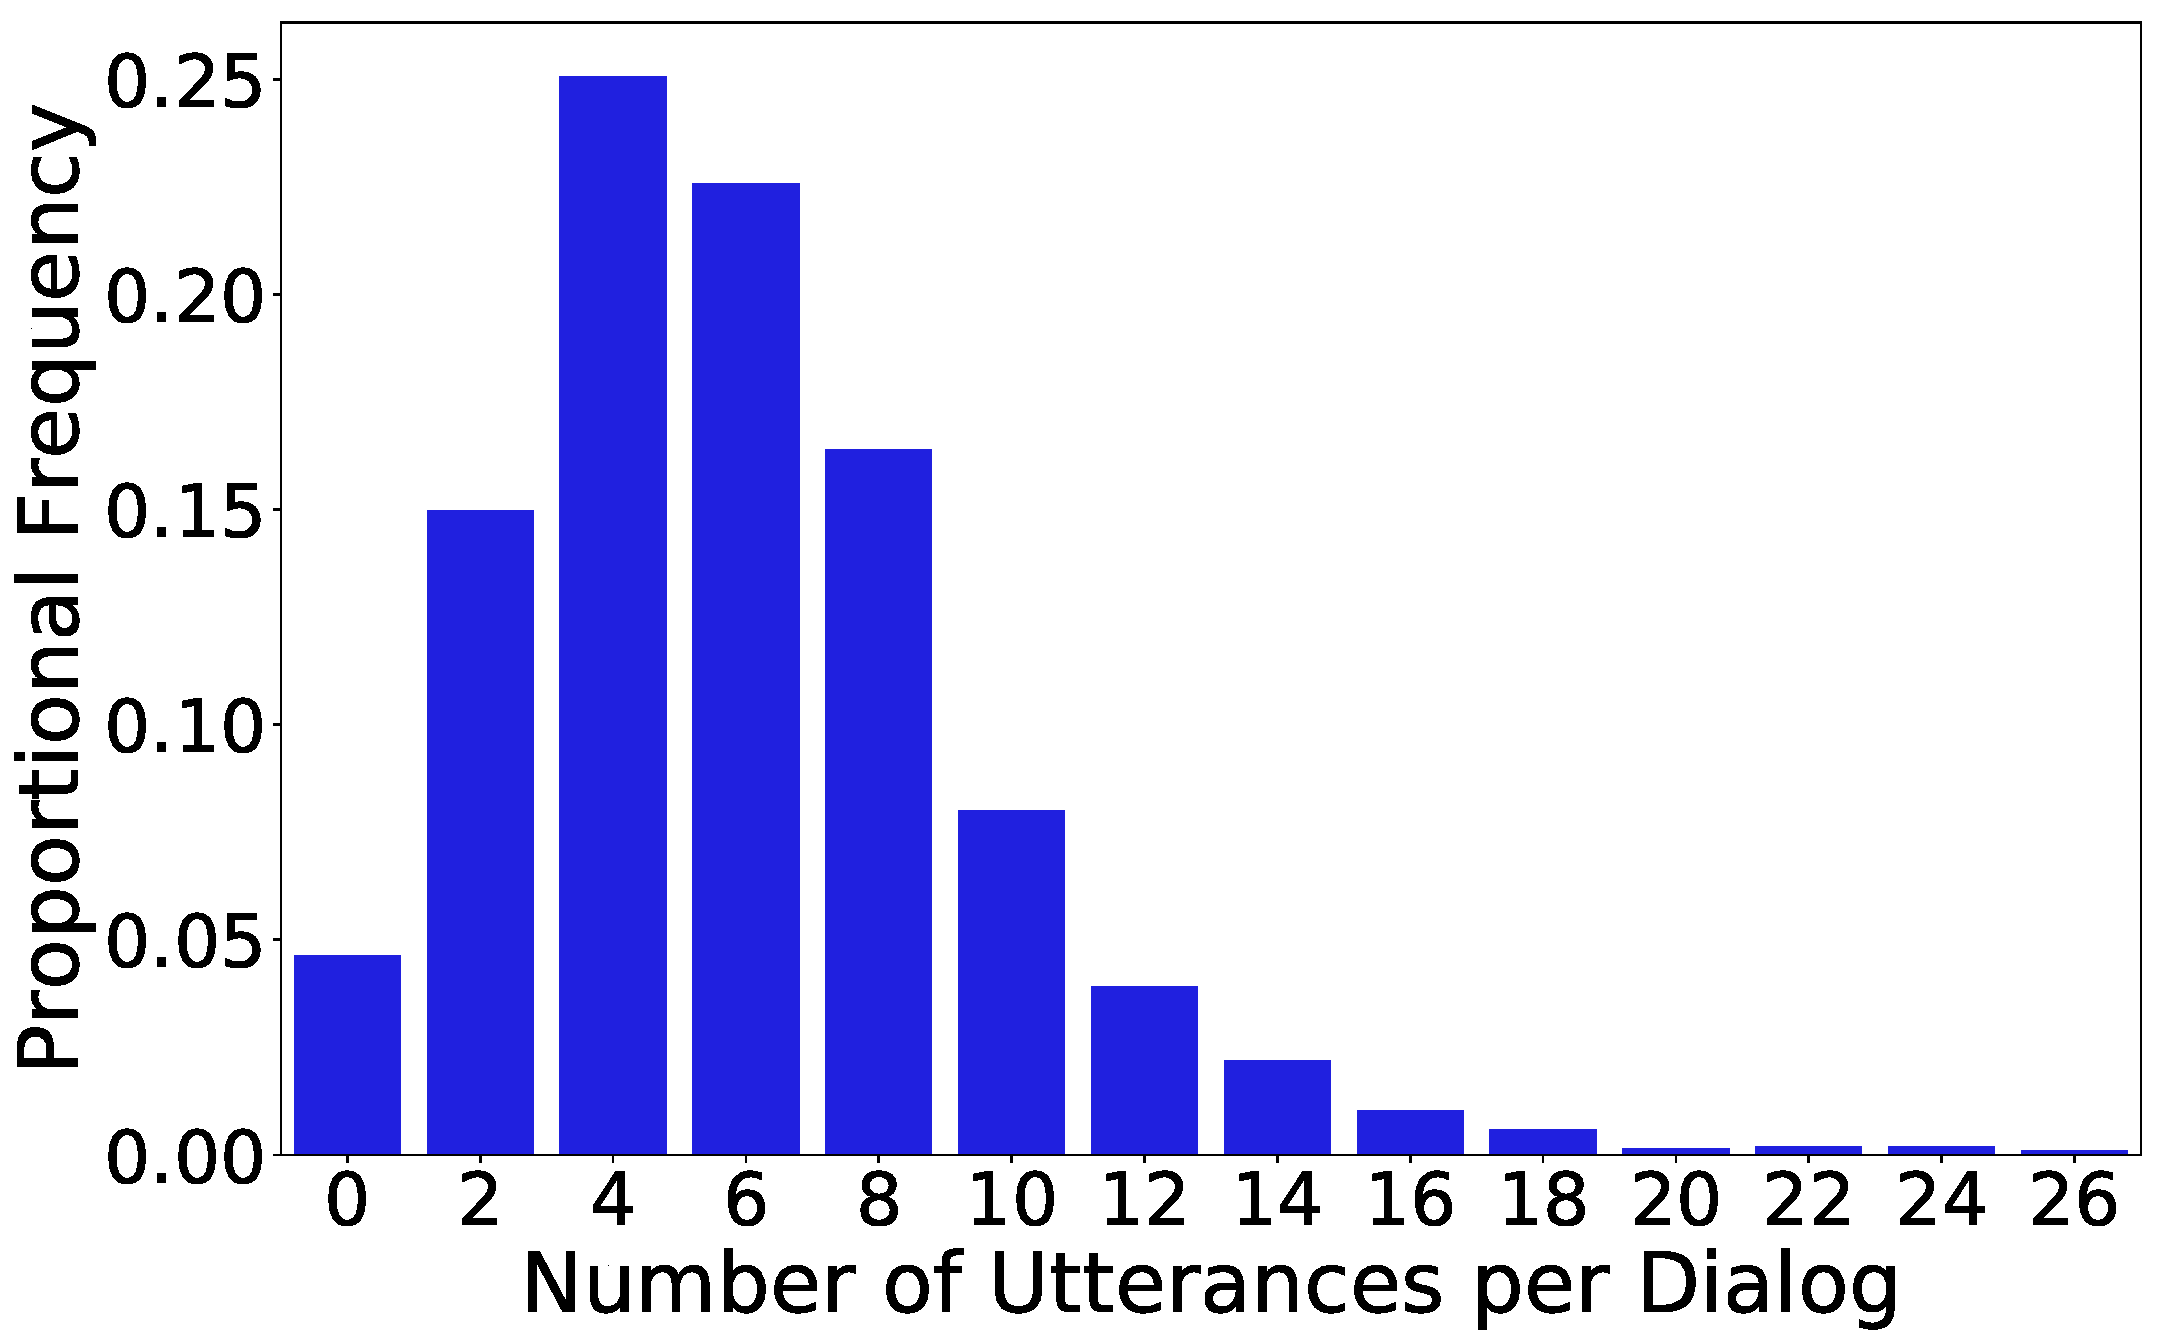
\includegraphics[width=0.3\columnwidth]{figures/utterances_per_dialog.pdf}
\end{tabular}
\caption{The distributions of steps taken by human \nav{}s versus a shortest path planner (Left), the number of word tokens from the \nav{} and the \ora{} (Center), and the number of utterances in dialogs across the \dataset{} dataset.}
\label{fig:steps_and_words}
\vspace{-4mm}
\end{figure}

\paragraph{Dialog Prompts.}
A dialog prompt is a tuple of the house scan $S$, a target object $t_o$ to be found, a starting position $p_0$, and a goal region $G_j$.
We use the MatterPort object segmentations to get region locations for household objects, as in prior work~\cite{nguyen:cvpr19}.
We define a set of 81 unique object types that appear in at least 5 unique houses and appear between 2 and 4 times per such house.\footnote{We also cut odd (``soffet'') and non-specific (``wall'') objects, and merge similar object names (e.g., ``potted plant'' and ``plant'') to cut down the initial 929 object types to these salient 81. Some houses do not have objects that meet our criteria, so \dataset{} represents only 83 of the 90 total MatterPort houses.}
Each dialog begins with a hint, such as ``The goal room contains a \textit{plant},'' which by construction is both ambiguous (there are two to four rooms with a plant) and underspecified (the path to the room is not described by the hint).

Given a house scan $S$ and a target object $t_o$, a dialog prompt is created for every goal region $G_j$ in the house containing an instance of $t_o$.
Goal regions are sets of nodes that occupy the same room in a house scan.
The starting node $p_0$ is chosen to maximize the distance between $p_0$ and the goal regions $G_{0:|G|}$ containing $t_o$.
Formally,
\begin{equation*}
    p_0 = \text{argmax}_{p\in S}\left(\sqrt{\sum_{j}{\min_{p_i\in G_j}(d_h(p, p_i)^2)}}\right).
\end{equation*}

\paragraph{Crowdsourced Data Collection.}
We gathered human-human dialogs through Amazon Mechanical Turk.\footnote{\url{https://cvdn.dev/}. Connect with two tabs to start a dialog with yourself.}
In each Human Intelligence Task (HIT), workers read about the roles of \nav{} and \ora{} and could practice using the navigation interface.
Pairs of workers were connected to one another via a chat interface.

Every dialog was instantiated via a randomly chosen prompt $(S, t_o, p_0, G_j)$, with the \nav{} starting at panorama $p_0$ and both workers instructed via the text: ``Hint: The goal room contains a $t_o$.''
The dialog begins with the \nav{}'s turn.
On the \nav{}'s turn, they could navigate, type a natural language question to ask the \ora{}, or guess that they had found the goal room.
Incorrect guesses disabled further navigation and forced the \nav{} to ask a question to the \ora{}.
Throughout navigation, the \ora{} was shown the steps being taken as a mirror of the \nav{}'s interface, so that both workers were always aware of the current visual frame.
On the \ora{}'s turn, they could view an animation depicting the next $5$ hops through the navigation graph towards the goal room according to a shortest path planner and communicate back to the \nav{} via natural language (Figure~\ref{fig:full_demo}).
Five hops was chosen because this is slightly shorter than the $6$ hop average path in the R2R dataset, for which human annotators were able to provide reasonable language descriptions.
Each HIT paid $\$1.25$ per worker, the entire dataset collection cost over \$7k.

After successfully locating the goal room, workers rated their partner's cooperativeness (from 1 to 5).
Workers who failed to maintain a 4 or higher average peer rating were disallowed from taking more of our HITs.
On average, dialog participants' mean peer rating is $4.52$ out of 5 across \dataset{}.

\paragraph{Analysis.}
The \dataset{} dataset has longer routes and language contexts than the R2R task.
The dialogs exhibit complex phenomena that require both dialog and navigation history to resolve.

\begin{table}[ht]
\centering
\begin{small}
\begin{tabular}{p{1.4cm}rrrp{8.5cm}}
    & \textbf{\textit{Dia}} & \textbf{\textit{Nav}} & \textbf{\textit{Ora}} & \textbf{Example} \\
    \toprule
    Ego & $92.5$ & $52.9$ & $65.8$ & \ora{}: Turn slightly to {\color{blue}your right} and go {\color{blue}forward} down the hallway \\
    \cmidrule{5-5}
    Needs Q & $13.0$ & - & $3.9$ & \nav{}: Should I turn left down the hallway ahead? \\
    & & & &  \ora{}: {\color{blue}ya} \\
    \cmidrule{5-5}
    Needs Dialog History & $3.5$ & $0.4$ & $1.0$ & \ora{}: Through the lobby. So go through the door next to the green towel. Go to the left door next to {\color{blue}the two yellow lights}. Walk straight to the end of the hallway and stop \\
    & & & & $\dots$ \\
    & & & & \nav{}: Are these {\color{blue}the yellow lights} you were talking about? \\
    \cmidrule{5-5}
    Needs Nav History & $14.0$ & $1.5$ & $3.4$ & \ora{}: {\color{blue}You were there briefly but left}. There is a turntable behind you a bit. Enter the bedroom next to it. \\
    \cmidrule{5-5}
    Repair & $12.5$ & $1.6$ & $3.4$ & \ora{}: I am so sorry {\color{blue}I meant for you to look over to the right not the left} \\
    \cmidrule{5-5}
    Off-topic & $3.0$ & $5.4$ & $5.1$ & \nav{}: I am to the `rear' of the zebra. {\color{blue}Nice one.} \\
    & & & & \ora{}: {\color{blue}Ok hold your nose} and go to the left of the zebra, through the livingroom and kitchen and towards the bedroom you can see past that \\
    \cmidrule{5-5}
    Vacuous & $6.0$ & $22.7$ & $2.3$ & \nav{}: {\color{blue}Ok, now where?} \\
    \bottomrule \\
\end{tabular}
\end{small}
\caption{
The average percent of \textit{Dia}logs, as well as individual \nav{} and \ora{} utterances, exhibiting each phenomena out of 100 hand-annotated dialogs.
Two authors annotated each dialog and reached an agreement of Cohen's~$\kappa=.738$ across all phenomena labels.
}
\vspace{-8mm}
\label{tab:analysis}
\end{table}

Figure~\ref{fig:steps_and_words} shows the distributions of path lengths, word counts, and number of utterances across dialogs in the \dataset{} dataset.
Human ($25.0\pm12.9$) and planner ($17.4\pm7.0$) path lengths are on average more than three times longer, and have higher variance, than the path lengths in R2R ($6.0\pm0.85$).
Average word counts for navigators ($33.5$) and oracles ($48.1$) sum to an average $81.6$ words per dialog, again exceeding the Room-to-Room average of $29$ words per instruction by nearly a factor of three.
Dialogs average about 6 utterances each (3 question and answer exchanges), with a fraction being much longer---up to 26 utterances.
Some dialogs have no exchanges (about 5\%): the \nav{} was able to find the goal location by intuition alone given the hint.
Because more than one room always contains $t_o$, these are `lucky' guesses.

We randomly sampled 100 dialogs with at least one QA exchange and annotated whether each utterance (out of 342 per speaker) exhibited certain phenomena (Table~\ref{tab:analysis}).
Over half the utterances from both \nav{} and \ora{} roles, and over 90\% of all dialogs, contain egocentric references requiring the agent's position and orientation to interpret.
Some \ora{} answers require the \nav{} question to resolve (e.g., when the answer is just a confirmation).
Some utterances need dialog history from previous exchanges or past visual navigation information.
More than 10\% of dialogs exhibit conversational repair, when speakers try to rectify mistakes.
Speakers sometimes establish rapport with off-topic comments and jokes.
Both speakers, especially those in the \nav{} role, sometimes send vacuous communications, but this is limited to a smaller percentage of dialogs.

Models attempting to perform navigation, ask questions, or answer questions about an embodied environment must grapple with these types of phenomena.
For example, an agent may need to attend not just to the last QA exchange, but to the entire dialog and navigation history in order to correctly follow instructions.
